\section{Distributionally Robust Counterfactuals}

We propose \textsc{LIFT-CF}, a distributional robustness wrapper for CF generators that operates \emph{post-hoc} on the population of CFs a generator produces, rather than modifying its objective or parameters.


Let $f_0: \mathcal{X}\to\{0,1\}$ be a binary classifier, with class $0$ unfavorable and class $1$ favorable, and let $G$ be a base CF generator. Given a batch $X=\{x_i\}_{i=1}^n$ of instances with $f_0(x_i)=0$, let $z_i = G(x_i)$ denote the corresponding CFs.
We represent the generated CF population by its empirical distribution
$
\mathbb{P}_{\mathrm{CF}} = \frac{1}{n}\sum_{i=1}^n \delta_{z_i},
$
and let $\mathbb{P}_1$ denote the empirical distribution of target-class training samples ($f_0(x)=1$).
The two distributions provide complementary information: $\mathbb{P}_{\mathrm{CF}}$ captures where the base generator currently places CFs, while $\mathbb{P}_1$ captures the observed structure of the favorable class. 
We use \emph{proximity} to denote closeness to $\mathbb P_{\mathrm{CF}}$, and \emph{plausibility} to denote alignment with $\mathbb P_1$. 
Note that $\mathbb P_{\mathrm{CF}}$ may resemble proximal CFs in the typical sense, i.e., close to the original instances, as we assume no prior knowledge about the base generator's internal objective.

Our goal is to refine $\mathbb P_{\mathrm{CF}}$ toward a region that remains robust to future shifts while preserving the generator's original CF structure.
This is a key distinction from instance-level methods (Section~\ref{sec:related}): rather than independently robustifying each CF, we seek a refined \emph{distribution} whose population-level geometry is robust to plausible future shifts, leaving the base generator itself unchanged.
%of its generated CFs through a Wasserstein lens-induced transport flow: $G$ remains responsible for producing CFs, and \textsc{LIFT-CF} refines their distributional robustness post hoc.


%Let $X=\{x_i\}_{i=1}^n$ be a batch of input instances with unfavorable outcomes, i.e., $f_0(x_i)=0$ for all $i$, and let
%$
%z_i = G(x_i), \quad i=1,\dots,n
%$
%be the corresponding CFs.% generated by $G$. 
%We represent the generated CF population by its empirical distribution
%$
%\mathbb{P}_{\mathrm{CF}} = \frac{1}{n}\sum_{i=1}^n \delta_{z_i}.
%$
%Let $\mathbb{P}_1$ denote the empirical distribution of target-class samples, i.e., training instances $x$ with $f_0(x)=1$. 
%These two distributions provide complementary information: $\mathbb{P}_{\mathrm{CF}}$ captures where the base generator currently places CFs, and $\mathbb{P}_1$ captures the observed structure of the favorable class. Throughout, we use \emph{proximity} to denote closeness to $\mathbb P_{\mathrm{CF}}$, and \emph{plausibility} to denote alignment with the observed target-class distribution $\mathbb P_1$. Note that $\mathbb P_{\mathrm{CF}}$ may resemble proximal counterfactuals in the typical sense, i.e., as close to the original instances as possible, but this is neither required nor can be assumed, as we do not have any prior knowledge about the CF generator itself.




\textbf{Overview.}
We formulate robust CF refinement in three steps. First, we construct a CF-induced Wasserstein lens capturing where the CF distribution should lie to remain valid under future shifts (Section~\ref{sec:lens}). Then, we show that a robust relaxation of the resulting minimax objective induces a one-dimensional Wasserstein barycentric family with provable risk bounds (Section~\ref{sec:barycentric}). Finally, we calibrate this refinement using held-out proxy deployment shifts (Section~\ref{sec:calibration}), and realize it via optimal transport (Section~\ref{sec:transport}).


\subsection{CF-Induced Wasserstein Lens}\label{sec:lens}

Data distributions evolve over time \citep{quionero2009dataset}, requiring the model to be retrained periodically. 
A CF $z_i = G(x_i)$ that is favorable under the current classifier $f_0$ does not necessarily remain favorable once $f_0$ is updated: a shift in the decision boundary may move $z_i$ back into the unfavorable region. 
Since the future classifier is unobserved at deployment time, we cannot hedge against a single predicted shift. 

Rather than modelling this uncertainty at the level of the classifier, e.g., positing a distribution over future model parameters or retraining updates, we model it directly at the level of the data: where the region of CFs lies in $\mathcal{X}$.
%This formulation is agnostic to how $f_0$ is retrained and instead captures the uncertainty purely in the space CFs already occupy.
This leads to a population-level rather than instance-level view of robustness.
Existing robustness methods hedge each $z_i$ individually. We instead ask: \emph{where should the distribution of generated CFs lie so that it remains compatible with plausible future target-class regions?} 
This shift in perspective requires an uncertainty set over future distributions rather than over individual CFs.

We model future distributions as bounded displacements of the distributions observable today. 
As data evolve, probability mass may move through $\mathcal{X}$, and Wasserstein-distance $W_2$ provides a natural notion of cost for such displacements. 
Formally, for a reference distribution $\mathbb{P}$ and radius $r\geq0$, define the Wasserstein ball $
B_{W_2}(\mathbb P,r)
=
\{\mu\in\mathcal P_2(\mathcal X): W_2(\mu,\mathbb P)\le r\},
$ which contains the distributions reachable from $\mathbb{P}$ with transport cost $\le r$. 
We regard $\mu\in B_{W_2}(\mathbb P,r)$ as a plausible future distribution for a suitable anchor $\mathbb{P}$ and radius $r$.


\textbf{Proximity vs. plausibility.}
None of the potential anchors $\mathbb{P}_0$, $\mathbb{P}_1$, and $\mathbb{P}_{\mathrm{CF}}$ is sufficient on its own to determine the future distribution of valid CFs. 
Anchoring only on the observed target-class distribution $\mathbb{P}_1$, a \emph{plausible} anchor, keeps the refinements close to the favorable class samples, but ignores the generator and its current CFs. Anchoring only on the empirical distribution $\mathbb{P}_{\mathrm{CF}}$, a \emph{proximal} anchor, keeps the refinement close to what the generator already produced, but does not include signal about proximity to class 1 samples. \emph{Moreover, these two anchors should not be viewed as independent sources of uncertainty: distributional shifts that alter the class population can simultaneously induce changes in the learned decision boundary, and hence in the location and validity geometry of the generated CFs.}
We thus impose both signals jointly: $\mathbb{P}_1$ as the only available evidence about the target-class structure, and $\mathbb{P}_{\mathrm{CF}}$ captures the generator-induced placement of currently valid CFs.

\textbf{The CF-induced lens.}
We build a \emph{lens} $\mathcal{C}$: a set of plausible future valid CF distributions, anchored on both complementary sources of evidence: the proximal and the plausible anchor.

We construct the CF-induced Wasserstein lens
\begin{equation}\label{eq:cf-inducedlens}
  \mathcal C
=
\left\{
\mu\in \mathcal{P}_2(\mathcal X):
W_2(\mu,\mathbb{P}_1)\le\epsilon,\;
W_2(\mu,\mathbb{P}_{\mathrm{CF}})\le\delta
\right\},  
\end{equation}
where $W_2$ denotes the 2-Wasserstein distance and $\mathcal{P}_2(\mathcal X)$ is the space of probability measures on $\mathcal{X}$ with finite second moments. 
Figure~\ref{fig:conceptual} shows this construction schematically: the lens is the intersection of two balls, one centered at $\mathbb{P}_{\mathrm{CF}}$ and one at $\mathbb{P}_1$.
%Here, $\mu$ represents a candidate distribution of target-class under a plausible future shift. 
The constraint $W_2(\mu,\mathbb{P}_1)\le\epsilon$ anchors $\mu$ to the \emph{observed} target-class structure. %, representing in-distribution samples and thus the plausible anchor.
The constraint $W_2(\mu,\mathbb{P}_{\mathrm{CF}})\le \delta$ reflects a \emph{CF-consistency} assumption: 
ruling out future CF distributions arbitrarily far from the generator's current CF region. %the current generator's CF $\mathbb{P}_{\mathrm{CF}}$ is the only signal about the generator's current counterfactual region, so we do not consider future target regions arbitrarily far from this signal anchoring the distribution to proximity. 
%Because our method is a post-hoc refinement of the current CF distribution generated by the base CF generator, the relevant future target-side distributions are those that remain compatible with the base generator's CFs.  
%Neither anchor alone is sufficient: $\mathbb{P}_1$ ignores the generator, while $\mathbb{P}_{\mathrm{CF}}$ alone would ignore the true target-class structure meant to recover. 
%The lens is therefore not intended to model the future distribution of counterfactuals themselves, but rather the set of plausible future target-side regions in which valid counterfactuals should remain embedded.
%\textcolor{frappe_red}{Neither anchor alone is sufficient: $\mathbb{P}_1$ ignores the generator, aiming at in-distribution CFs only and disregarding proximity, thus often reflecting larger and less actionable changes than necessary, while $\mathbb{P}_{\mathrm{CF}}$ alone would ignore the true target-class structure meant to recover, and might face validity issues under shift.}

\begin{proposition}[Wasserstein proximity--plausibility trade-off]\label{prop:cf-tradeoff}
Let $D
=
W_2(\mathbb{P}_{\mathrm{CF}},\mathbb{P}_1)$
and let $\{\mathbb{P}^{\mathrm{geo}}_t\}_{t\in[0,1]}$ be any constant-speed $W_2$-geodesic connecting $\mathbb{P}_{\mathrm{CF}}$ and $\mathbb{P}_1$, with
$\{\mathbb{P}^{\mathrm{geo}}_0\}=\mathbb{P}_{\mathrm{CF}}$ and $\{\mathbb{P}^{\mathrm{geo}}_1\}=\mathbb{P}_{1}$. Then, for every $t\in[0,1]$, $$W_2(\mathbb{P}^{\mathrm{geo}}_t,\mathbb{P}_{\mathrm{CF}})=tD, \qquad W_2(\mathbb{P}^{\mathrm{geo}}_t,\mathbb{P}_{\mathrm{1}})=(1-t)D.$$
Consequently, a point $\mathbb{P}^{\mathrm{geo}}_t \in \mathcal{C}= B_{W_2}(\mathbb{P}_{\mathrm{CF}},\delta)\cap B_{W_2}(\mathbb{P}_1,\epsilon)$
if $tD\leq\delta$ and $(1-t)D\leq\epsilon$, i.e.,
$$t \in \left[
1-\frac{\epsilon}{D},
\frac{\delta}{D}
\right]
\cap[0,1].$$
Along the geodesic, $t$ is thus an explicit proximity-plausibility parameter: increasing $t$ increases displacement from $\mathbb{P}_{\mathrm{CF}}$ while decreasing the displacement from $\mathbb{P}_1$, with  radii $\delta$ and $\epsilon$ controlling the maximum admissible proximity displacement from each anchor respectively.
The lens contains a point on the geodesic if $\epsilon+\delta \geq D$.
When equality holds, the interval collapses to the unique parameter $t^* =\frac{\delta}{D} = 1- \frac{\epsilon}{D},$
which satisfies both constraints.
\end{proposition}

Proposition~\ref{prop:cf-tradeoff} gives the lens a direct geometric interpretation.: along the Wasserstein path between two anchors, increasing the path parameter moves the candidate future distribution away from $\mathbb{P}_{\mathrm{CF}}$ and towards $\mathbb{P}_{1}$ . 
Hence, $\epsilon$ and $\delta$ do not constitute independent notions of plausibility and proximity; they jointly constrain the size of the uncertainty set.
Crucially, $\mathcal C$ does not assume access to the actual future distribution, where $\epsilon,\delta\ge0$ specify an admissible nonempty lens.
%The radii $\epsilon$ and $\delta$ determine the admissible extent of distributional displacement from the two complementary anchors.
%In particular, Proposition~\ref{prop:cf-tradeoff} formalizes the resulting proximity-plausibility trade-off along the Wasserstein path connecting $\mathbb{P}_{\mathrm{CF}}$ and $ \mathbb{P}_1$.
We assume throughout that $\mathcal{C}\neq\emptyset$, which by Proposition~\ref{prop:cf-tradeoff} holds when
$\epsilon+\delta\ge
W_2(\mathbb{P}_{\mathrm{CF}},\mathbb{P}_1)$.
%The radii $\epsilon$ and $\delta$ determine the size of the uncertainty set and the value of the resulting robust certificate, but, as shown below (Section~\ref{sec:barycentric}),do not determine the barycentric search direction induced by the robust relaxation. We assume that $\mathcal{C}\neq\emptyset$. In the present Wasserstein setting, this is ensured when $\epsilon+\delta\geW_2(\mathbb{P}_{\mathrm{CF}},\mathbb{P}_1)$.
%Instead, $\epsilon$ and $\delta$ are calibrated using held-out proxy shifts (Section~\ref{sec:calibration}) to cover a prescribed fraction of candidate future-valid CF distributions; we also verify there that $\epsilon + \delta \ge W_2(\mathbb{P}_{\mathrm{CF}}, \mathbb{P}_1)$, which keeps $\mathcal{C}$ nonempty by the triangle inequality.
%The lens does not assume access to the actual future distribution; instead, its radii are calibrated using held-out proxy shifts to cover a prescribed fraction of candidate future-valid CF distributions.
%The lens contains distributions that are simultaneously close to the observed target-class distribution $\mathbb{P}_1$ and the initial CF distribution $\mathbb{P}_{\mathrm{CF}}$. The two distributions provide complementary anchors: $\mathbb{P}_1$ represents the observed target-class structure, whereas $\mathbb{P}_{\mathrm{CF}}$ represents the output of the base CF generator. 
%The radii $\epsilon$ and $\delta$ are calibrated using held-out proxy deployment shifts, thereby giving the lens an empirical future-shift interpretation.

\textbf{Robustness.}
Robustness is measured by requiring the refined CF distribution $\mathbb{Q}$ to stay close to every plausible future CF distribution $\mu$ in the lens. 
For any candidate $\mathbb{Q}\in\mathcal \mathcal{P}_2(\mathcal X)$, we define its worst-case lens risk as
\begin{equation}
   \label{eq:worstcaserisk}
R(\mathbb{Q})
=
\sup_{\mu\in\mathcal C}W_2^2(\mathbb{Q},\mu). 
\end{equation} 
\emph{Since the CF distribution required under a future deployment may lie anywhere within the lens, we seek a distribution $\mathbb{Q}$ that minimizes its worst-case distance to all admissible locations.}
A smaller $R(\mathbb{Q})$ indicates a smaller worst-case
distributional mismatch over the uncertainty lens.



\subsection{Robust-Bound-Induced Barycentric Geometry}\label{sec:barycentric}

Directly solving
\begin{equation}
   \label{eq:intractable_objective}
\min_{\mathbb{Q}\in  \mathcal{P}_2(\mathcal X)}
R(\mathbb{Q})
=
\min_{\mathbb{Q}\in  \mathcal{P}_2(\mathcal X)}
\sup_{\mu\in\mathcal C}W_2^2(\mathbb{Q},\mu)
\end{equation} 
is generally intractable, since it requires solving an inner supremum over $\mathcal C$ for every candidate $\mathbb{Q}$. 
We instead minimize a tractable family of valid upper bounds on $R(\mathbb{Q})$. 
The key consequence is that the resulting upper bounds induce a two-anchor Wasserstein barycentric family: Proposition~\ref{prop:cf-tradeoff} already establishes the proximity-plausibility geometry of the path, and the result below shows that the robust relaxation selects candidates precisely from this geometry.

%each bound's minimizer lies on the Wasserstein barycentric path connecting the original counterfactual distribution
%$\mathbb{P}_{\mathrm{CF}}$ and the observed target distribution $\mathbb{P}_1$.

\begin{proposition}[Robust-bound-induced barycentric family]
\label{prop:barycentric_family}
Given the lens $\mathcal{C}$ in Eq.~\ref{eq:cf-inducedlens},
there exists a family of valid upper bounds on the worst-case risk
$R(\mathbb{Q})$ whose minimizers take the form
\begin{equation}
(1-\lambda)
W_2^2(\mathbb{Q},\mathbb{P}_{\mathrm{CF}})
+
\lambda
W_2^2(\mathbb{Q},\mathbb{P}_1),
\qquad
\lambda\in[0,1].
\label{eq:barycentric_family}
\end{equation}
The minimizers of these relaxed bounds form the two-anchor Wasserstein family
%Moreover, the induced barycentric weight spans the entire interval
%$[0,1]$. Hence the robust relaxation induces the one-dimensional
%family
$\
\mathcal{Q}
:=
\left\{
\mathbb{Q}(\lambda):\lambda\in[0,1]
\right\},
\label{eq:barycentric_path}
$
where
\begin{equation}
\mathbb{Q}(\lambda)
\in
\arg\min_{\mathbb{Q}\in\mathcal{P}_2(\mathcal X)}
\left\{
(1-\lambda)W_2^2(\mathbb{Q},\mathbb{P}_{\mathrm{CF}})
+
\lambda W_2^2(\mathbb{Q},\mathbb{P}_1)
\right\},
\label{eq:barycentric_family2}
\end{equation}
with endpoints $\mathbb{Q}(0)=\mathbb{P}_{\mathrm{CF}}$ and $\mathbb{Q}(1)=\mathbb{P}_1$.
\end{proposition}
\begin{figure}[t]
    \centering
    %  left bottom right top
    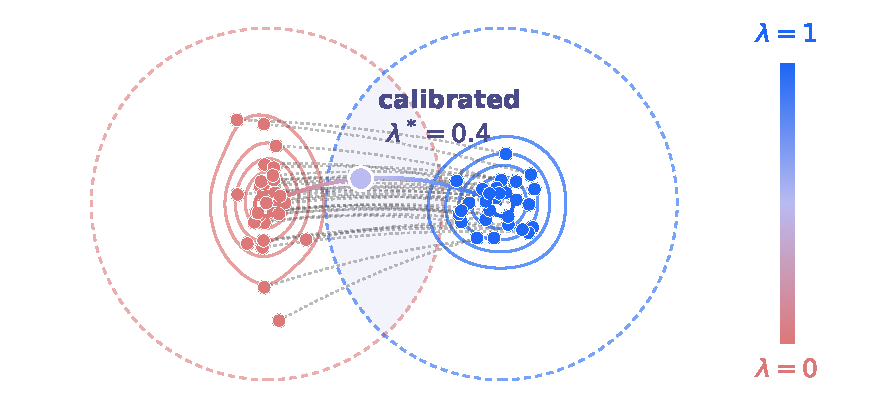
\includegraphics[trim={1.5cm 0.4cm 0.9cm 0.4cm},clip,width=0.45\linewidth]{Figures/conceptual_sketch_tradeoff_compact.pdf}
    \caption{\textbf{Certified lens and optimal-transport coupling.} The dashed ellipses show the certified lens $\mathcal{C}$, centered at base CF-distribution $\mathbb{P}_{\mathrm{CF}}$ (pink) and observed target-class distribution $\mathbb{P}_1$ (teal) with radii $\delta$ and $\epsilon$. The shaded intersection is $\mathcal{C}$. Dashed lines show the optimal coupling $\pi^\star$ between the two empirical distributions, and the purple marker shows the calibrated barycenter $\mathbb{Q}(\lambda^\star)$ realized along this coupling, positioned inside the lens.}
    \label{fig:conceptual}
\end{figure}

\textbf{Proof sketch.}
For any $\mu\in\mathcal{C}$, the lens constraints and triangle
inequality give
$
W_2(\mathbb{Q},\mu)
\le
\min\!\left\{
W_2(\mathbb{Q},\mathbb{P}_{\mathrm{CF}})+\delta,\,
W_2(\mathbb{Q},\mathbb{P}_1)+\epsilon
\right\}.
$
A convex relaxation followed by Young's inequality yields a family
of valid upper bounds whose $\mathbb{Q}$-dependent terms are positive
weighted sums of
$W_2^2(\mathbb{Q},\mathbb{P}_{\mathrm{CF}})$ and
$W_2^2(\mathbb{Q},\mathbb{P}_1)$.
After normalization, their minimizers take the barycentric form in
Eq.~\ref{eq:barycentric_family}.
The admissible bounds span $\lambda\in[0,1]$.
See Appendix~\ref{app:barycentric_bound} for the full proof.

Proposition~\ref{prop:barycentric_family} certifies a family of candidates, not a single optimum: each $\mathbb{Q}(\lambda)$ minimizes a valid upper bound on $R(\mathbb{Q})$, but the proposition does not claim that any $\mathbb{Q}(\lambda)$  minimizes $R(\mathbb{Q})$ itself, nor that the bound is tight. 
%Proposition~\ref{prop:barycentric_family} does not assert that every
%$\mathbb{Q}(\lambda)$ directly minimizes the original worst-case risk
%$R(\mathbb{Q})$. Rather, it shows that the lens induces a family of
%\emph{certified barycentric candidates}, each minimizing a valid
%upper bound on $R(\mathbb{Q})$. 
The remaining question is therefore not where to search for a robust refinement, but where to locate the refinement along this certified path, a choice we calibrate in Section~\ref{sec:calibration}.%

% \begin{corollary}[Geodesic characterization and conditional uniqueness]
% \label{cor:geodesic_characterization}
% Let $D=W_2(\mathbb{P}_{\mathrm{CF}},\mathbb{P}_1)$.
% At the endpoints, $\mathbb{Q}(0)= \mathbb{P}_\mathrm{CF}$ and $\mathbb{Q}(1)= \mathbb{P}_\mathrm{1}$ trivially.
% For any $\lambda\in(0,1)$, every minimizer of Eq.~\ref{eq:barycentric_family} lies at time $\lambda$ on a constant-speed $W_2$ geodesic between $\mathbb{P}_{\mathrm{CF}}$ and $\mathbb{P}_1$. In particular,
% \begin{equation}
% W_2(\mathbb{Q}(\lambda),\mathbb{P}_{\mathrm{CF}})
% =
% \lambda D,
% \qquad
% W_2(\mathbb{Q}(\lambda),\mathbb{P}_1)
% =
% (1-\lambda)D.
% \label{eq:geodesic_distances}
% \end{equation}
% Conversely, every time-$\lambda$ point on such a geodesic minimizes Eq.~\ref{eq:barycentric_family}.
% If the optimal coupling between $\mathbb{P}_{\mathrm{CF}}$ and $\mathbb{P}_1$ is unique, then $\mathbb{Q}(\lambda)$ is unique for every $\lambda\in(0,1)$, and the bound family induces a unique displacement path between the two anchors. 
% Thus, the barycentric parameter $\lambda$ coincides with the proximity--plausibility parameter of Proposition~\ref{prop:cf-tradeoff}.
% \end{corollary}

% Combining Corollary~\ref{cor:geodesic_characterization} with Proposition~\ref{prop:cf-tradeoff} gives
% \begin{equation}
% \mathbb{Q}(\lambda)\in\mathcal{C}
% \quad\Longleftrightarrow\quad
% \lambda D\leq\delta
% \;\text{ and }\;
% (1-\lambda)D\leq\epsilon,
% \label{eq:barycentric_lens_membership}
% \end{equation}
% or equivalently,
% $\lambda
% \in
% \left[
% 1-\frac{\epsilon}{D},
% \frac{\delta}{D}
% \right]\cap[0,1]$.



\textbf{Geometry versus certificate.}
The two anchors $\mathbb{P}_{\mathrm{CF}}$ and $\mathbb{P}_1$ determine the \emph{direction} of the barycentric refinement, $\lambda=0$ recovers the original CF distribution, $\lambda=1$ gives full alignment with target class distribution, and intermediate values trade off generator specific CF geometry against target-side alignment.
The lens radii $\epsilon$ and $\delta$ instead govern calibration risk: they determine the admissible proximity-plausibility range and the resulting robust certificates, without affecting which geodesic the refinement moves along. 
The decoupling matters in operation: it means that the search direction is fixed by the generator and the data as soon as $G$ and $\mathbb{P}_1$ are given, while the choice of \emph{where} along that direction to certify is a separate, data-driven calibration problem.
Certification of the entire path does not imply every $\lambda$ is equally desirable; it identifies a theoretically justified search family, not an operating point, since the two anchors alone cannot determine the future distribution that $\mathbb{P}_1$ only approximates.
We thus use held-out proxy deployment shifts to select $\lambda^\star$ along the certified path.

%In particular, Proposition~\ref{prop:cf-tradeoff} characterizes how $\epsilon$ and $\delta$ constrain the Wasserstein path between $\mathbb{P}_{\mathrm{CF}}$ and $\mathbb{P}_1$, whereas Proposition~\ref{prop:barycentric_family} shows that the robust relaxation induces candidates along this two-anchor path. Thus, the radii determine the admissible uncertainty and certificate, while the anchors determine the candidate refinement geometry.
%The lens radii $\epsilon$ and $\delta$ affect the value and tightness of the resulting robust upper bounds, but not their $\mathbb{Q}$-dependent minimization geometry. In particular, the radii enter the additive certificate terms in the bound, whereas the two anchors determine the barycentric geodesic characterized above. Thus, Proposition~\ref{prop:barycentric_family} should not be interpreted as claiming that $\mathbb{Q}(\lambda)$ solves the original minimax problem in Eq.~\ref{eq:intractable_objective}. Rather, the robust analysis reduces the unrestricted search over $\mathcal{P}_2(\mathcal X)$ to a one-dimensional, two-anchor barycentric candidate geometry.

%The endpoints have a direct interpretation:
%$\lambda=0$ recovers the original CF distribution
%$\mathbb{P}_{\mathrm{CF}}$, whereas $\lambda=1$ corresponds to full
%alignment with the observed target distribution $\mathbb{P}_1$.
%Intermediate values trade off preservation of the generator-specific
%counterfactual geometry against target-side alignment. 
%Certification of the entire path does not imply that all values of $\lambda$ are equally desirable; it identifies a theoretically justified search
%family, while the appropriate operating point depends on deployment
%evidence. The two anchors alone cannot determine this operating point:
%$\mathbb{P}_{\mathrm{CF}}$ reflects the current generator, whereas
%$\mathbb{P}_1$ reflects the observed target population rather than
%the unknown future one. We therefore use held-out proxy deployment
%shifts in Section~\ref{sec:calibration} to select
%$\lambda^\star$ along the certified path.

% \subsection{Deployment Calibration along the Certified Path}
% \label{sec:calibration}

% We use a held-out calibration set containing $M$ proxy deployment
% environments. Let $\widehat{\mu}_m$, $m=1,\ldots,M$, denote the
% target-side reference distribution under the $m$-th proxy shift.
% These calibration distributions are used only for calibration and
% are disjoint from the shifted environments used for final evaluation.

%\textbf{Lens calibration.}
%For a user-specified miscoverage level $\alpha_{\mathrm{cal}}\in(0,1)$, we calibrate the two lens radii using empirical distance quantiles:
%\begin{equation}\label{eq:radii_calibration}
%\delta
%=
%\operatorname{Quantile}_{1-\alpha_{\mathrm{cal}}}
%\left(
%\left\{
%W_2(\widehat{\mu}_m,\mathbb{P}_{\mathrm{CF}})
%\right\}_{m=1}^M
%\right),
% \quad
% \epsilon
% =
% \operatorname{Quantile}_{1-\alpha_{\mathrm{cal}}}
% \left(
% \left\{
% W_2(\widehat{\mu}_m,\mathbb{P}_1)
% \right\}_{m=1}^M
% \right).
% \end{equation}
% By construction, each radius individually covers a ($1-\alpha_{\mathrm{cal}}$) fraction of the proxy deployment distributions with respect to its own anchor. By a union bound, the lens $\mathcal{C}$ jointly covers at least a $(1-2\alpha_{\mathrm{cal}})$ fraction.
% %Thus, the lens is calibrated to cover a prescribed fraction of the
% %proxy deployment distributions. 
% We additionally enforce
% $
% \epsilon+\delta
% \ge
% W_2(\mathbb{P}_{\mathrm{CF}},\mathbb{P}_1)
% $
% to ensure that the lens is nonempty.

% \textbf{Path calibration.}
% Proposition~\ref{prop:barycentric_family} reduces the refinement
% search to the certified barycentric family
% $\{\mathbb{Q}(\lambda):\lambda\in[0,1]\}$.
% We select the member that minimizes the worst-case mismatch over the
% held-out proxy shifts:
% \begin{equation}
% \widehat{R}_{\mathrm{cal}}(\lambda)
% :=
% \max_{m=1,\ldots,M}
% W_2^2\!\left(
% \mathbb{Q}(\lambda),\widehat{\mu}_m
% \right),
% \label{eq:proxy_risk}
% \end{equation}
% \begin{equation}
% \lambda^\star
% \in
% \arg\min_{\lambda\in[0,1]}
% \widehat{R}_{\mathrm{cal}}(\lambda).
% \label{eq:lambda_calibration}
% \end{equation}
% The resulting $\mathbb{Q}(\lambda^\star)$ is therefore the member of the certified barycentric family that is most robust to the observed proxy deployment shifts. 
% Importantly, the proxy shifts used for this selection are held out from the final evaluation environments.

\iffalse
\subsection{Deployment-Stress Calibration}
\label{sec:calibration}

Section~\ref{sec:barycentric} reduces the unrestricted refinement problem to the one-dimensional barycentric family $\{\mathbb{Q}(\lambda):\lambda\in[0,1]\}$, whose parameter $\lambda$ has the exact proximity--plausibility interpretation established in Proposition~\ref{prop:cf-tradeoff}.
The robust analysis therefore determines a theoretically justified candidate geometry, but does not prescribe which operating point along this path should be deployed.
Since the realized deployment shift is unknown at construction time, we select the operating point using held-out calibration factuals evaluated under radius-specific adversarial model updates constructed from the training split.

% \textbf{Calibration stresses.}
% We construct $M$ stressed calibration datasets 
% $\mathcal{D}_{\mathrm{cal}}^{(m)}=\left\{\xi_i+\Delta_i^{(m)}\right\}_{i=1}^{N}$,
% $m=1,\ldots,M$ from a held-out split $\mathcal{D}_{\mathrm{cal}}=\{\xi_i\}_{i=1}^{N}$,
% where each perturbation satisfies a common transport budget $\frac{1}{N}\sum_{i=1}^{N}\left\|\Delta_i^{(m)}\right\|_2^2 \le b_{\mathrm{cal}}^2$.
% We set $b_{\mathrm{cal}}$ via a standard bootstrap procedure: letting $\widehat{\mathbb{P}}_{\mathrm{cal}}=\frac{1}{N}\sum_{i=1}^{N}\delta_{\xi_i}$ be the empirical calibration distribution and $\widehat{\mathbb{P}}_{\mathrm{cal}}^{*(r)}$,$r=1,\dots,B$ its bootstrap resamples,
% \begin{equation}
% b_{\mathrm{cal}}
% =
% \operatorname{Quantile}_{1-\alpha}
% \left\{
% W_2\!\left(
% \widehat{\mathbb{P}}_{\mathrm{cal}}^{*(r)},
% \widehat{\mathbb{P}}_{\mathrm{cal}}
% \right)
% \right\}_{r=1}^{B}.
% \label{eq:bootstrap_budget}
% \end{equation}
% This gives an evaluation-free reference scale for local stresses; it is not an estimate of the realized future distribution shift.


\textbf{Held-out calibration.}
We use a held-out split
$\mathcal{D}_{\mathrm{cal}}=\{\xi_i\}_{i=1}^{N}$
only to select refinement operating points for robustness configurations
constructed from the training split. In particular, the calibration data are
not used to construct an additional ambiguity set, generate new
distributional stresses, or update the corresponding adverse models.
All adverse model-update configurations and refinement geometries are frozen
before the calibration split is accessed. We first restrict calibration to factual instances that are unfavorable under
the current classifier,
$
\mathcal{I}_{\mathrm{cal}}
:=
\left\{
i:
f_0(x_i^{\mathrm{cal}})<\tau
\right\}.
$
For each $i\in\mathcal{I}_{\mathrm{cal}}$, the unchanged base generator
produces
$
z_i^{\mathrm{cal}}
=
G(x_i^{\mathrm{cal}}).
$
Only successful CFs satisfying
$f_0(z_i^{\mathrm{cal}})\geq\tau$
are retained. For a candidate refinement depth $\lambda$, each retained
base CF is refined using the same frozen rule as in training,
$
z_i^{\mathrm{cal}}(\lambda)
=
\operatorname{Refine}_{\lambda}
\bigl(z_i^{\mathrm{cal}}\bigr).
$
No model is updated at this stage; the refined calibration CFs are evaluated
under adverse model-update configurations constructed exclusively from the
training split.

\textbf{Within-radius operating-point calibration.}
For each uncertainty radius $r\in\mathcal{R}$, let
$\mathcal{F}_{r}^{\mathrm{adv}}$
denote the corresponding frozen family of adverse fine-tuned models. We define
the held-out calibration invalidity at refinement depth $\lambda$ as
\begin{equation}
\widehat L_{\mathrm{cal}}(r,\lambda)
:=
\max_{f\in\mathcal{F}_{r}^{\mathrm{adv}}}
\frac{1}{|\mathcal{I}_{\mathrm{cal}}^{\mathrm{valid}}|}
\sum_{i\in\mathcal{I}_{\mathrm{cal}}^{\mathrm{valid}}}
\left[
\tau
-
f\!\left(
z_i^{\mathrm{cal}}(\lambda)
\right)
\right]_+ ,
\label{eq:heldout_calibration_invalidity}
\end{equation}
where
$\mathcal{I}_{\mathrm{cal}}^{\mathrm{valid}}$
contains the calibration factuals for which the base generator returns a
current-valid CF. Together with the corresponding recourse cost
$C_{\mathrm{cal}}(\lambda)$, this defines, for each fixed $r$, a
robustness--proximity trade-off over $\lambda$. A predefined frontier
operating-point rule selects
\[
\lambda_r^\star
\in
\operatorname{SelectFrontier}
\left\{
\bigl(
C_{\mathrm{cal}}(\lambda),
\widehat L_{\mathrm{cal}}(r,\lambda)
\bigr)
:
\lambda\in\Lambda
\right\},
\]
where lower recourse cost and lower calibration invalidity are preferred.

\textbf{Cross-radius validation.}
The resulting configurations
$\{(r,\lambda_r^\star):r\in\mathcal{R}\}$
are subsequently evaluated on a disjoint shift-validation set whose
realizations are not used in the within-radius selection of
$\lambda_r^\star$. This second stage compares uncertainty coverage against
held-out robustness across radii and selects the final radius
$r^\star$ using a predefined coverage--validity trade-off rule. The deployed
refinement depth is then fixed as
$\lambda_{r^\star}^\star$.
No information from the final future-shift test set is used in either the
within-radius calibration of $\lambda$ or the cross-radius selection of $r$.
%Let
%$\mathcal{D}_{\mathrm{cal}}=\{\xi_i\}_{i=1}^{N}$
%denote a held-out calibration split that is not used for evaluation.
%We construct $M$ stressed calibration datasets
%\begin{equation}
%\mathcal{D}_{\mathrm{cal}}^{(m)}
%=
%\left\{
%\xi_i+\Delta_i^{(m)}
%\right\}_{i=1}^{N},
%\qquad
%m=1,\ldots,M,
%\label{eq:calibration_stresses}
%\end{equation}
%where each perturbation satisfies the common transport budget
%\begin{equation}
%\frac{1}{N}
%\sum_{i=1}^{N}
%\left\|
%\Delta_i^{(m)}
%\right\|_2^2
%\le
%b_{\mathrm{cal}}^2.
%\label{eq:calibration_budget}
%\end{equation}
%Here, $b_{\mathrm{cal}}$ is a data-dependent local stress scale, not an estimate of the magnitude or direction of the realized future deployment shift.

%\textbf{Data-driven stress scale.}
%We determine $b_{\mathrm{cal}}$ exclusively from $\mathcal{D}_{\mathrm{cal}}$, without access to any evaluation shift.
%Let
%\[
%\widehat{\mathbb{P}}_{\mathrm{cal}}
%=
%\frac{1}{N}
%\sum_{i=1}^{N}
%\delta_{\xi_i}
%\]
%denote the empirical calibration distribution, and let
%$\widehat{\mathbb{P}}_{\mathrm{cal}}^{*(r)}$,
%$r=1,\ldots,B$, denote empirical distributions obtained from
%bootstrap resamples of $\mathcal{D}_{\mathrm{cal}}$.
%We set
% \begin{equation}
% b_{\mathrm{cal}}
% =
% \operatorname{Quantile}_{1-\alpha}
% \left\{
% W_2\!\left(
% \widehat{\mathbb{P}}_{\mathrm{cal}}^{*(r)},
% \widehat{\mathbb{P}}_{\mathrm{cal}}
% \right)
% \right\}_{r=1}^{B}.
% \label{eq:bootstrap_budget}
% \end{equation}
%Thus, bootstrap variability is used only to establish an evaluation-free reference scale for local stresses; it is not used to predict the realized future distribution shift or to select $\lambda$ directly.

% \textbf{Proxy deployment models.}
% Within this budget, we generate stress directions $\Delta^{(1)},\ldots,\Delta^{(M)}$ and retrain the predictive model on each stressed datasets using the original training procedure, 
% %This yields
% $
% f^{(m)}
% =
% \operatorname{Train}
% \left(
% \mathcal{D}_{\mathrm{train}}
% \cup
% \mathcal{D}_{\mathrm{cal}}^{(m)}
% \right)$,
% %\qquad
% $m=1,\ldots,M$,
% %\label{eq:proxy_models}
% %\end{equation}
% with the stress-generation procedure detailed in Section~\textcolor{latte_maroon}{add label}\ref{sec:experimental_setup}.
% %where the precise stress-generation procedure is given in Section~\ref{sec:experimental_setup}.
% The resulting models $f^{(1)},\ldots,f^{(M)}$ are not predictions of the realized future classifier, but proxies that probe the sensitivity to controlled local model updates.
% %Rather, they serve as proxy deployment models that probe the
% %sensitivity of candidate refinements to controlled local model
% %updates.

% \textbf{Operating-point selection.}
% For each candidate $\lambda$, we evaluate the corresponding barycentric distribution $\mathbb{Q}(\lambda)$ under all $M$ proxy models. %deployment shifts. 
% Using the margin-based invalidity surrogate $\ell_f(z)
% =
% [\tau-f(z)]_+$, 
% %\begin{equation}
% %\ell_f(z)
% %=
% %[\tau-f(z)]_+,
% %\label{eq:calibration_loss}
% %\end{equation}
% we define the worst-case calibration risk
% \begin{equation}
% \widehat{R}_{\mathrm{cal}}(\lambda)
% =
% \max_{m\in[M]}
% \mathbb{E}_{z\sim\mathbb{Q}(\lambda)}
% \left[
% \ell_{f^{(m)}}(z)
% \right].
% \label{eq:calibration_risk}
% \end{equation}
% Lower values of $\widehat{R}_{\mathrm{cal}}(\lambda)$ indicate greater robustness to the deployment shifts.


\iffalse
Importantly, we do not select $\lambda$ by minimizing $\widehat{R}_{\mathrm{cal}}(\lambda)$ alone:
this can favor large values of $\lambda$, since moving toward the target anchor may keep improving robustness while incurring increasingly large departures from the proximal anchor. 
Instead, using the geodesic characterization in $W_2\!\left(
\mathbb{Q}(\lambda),
\mathbb{P}_{\mathrm{CF}}
\right)
=
\lambda D$ (with $D
:=
W_2(\mathbb{P}_{\mathrm{CF}},\mathbb{P}_1)$), 
so $\lambda$ itself is the normalized refinement depth, we select an operating point on the
robustness--refinement frontier.

%Section~\ref{sec:barycentric} to make this additional refinement
%explicit. Since
%$
%D
%:=
%W_2(\mathbb{P}_{\mathrm{CF}},\mathbb{P}_1),
%$
%along the barycentric path,
%$
%W_2\!\left(
%\mathbb{Q}(\lambda),
%\mathbb{P}_{\mathrm{CF}}
%\right)
%=
%\lambda D,
%\label{eq:refinement_cost}
%$
%$\lambda$ itself is the normalized refinement depth from the proximal anchor.
%We therefore select an operating point on the
%robustness--refinement frontier rather than the point of maximal robustness. %Specifically, relative to the unrefined counterfactual
We define the normalized robustness gain relative to the unrefined CF population,
% population, define the normalized robustness gain
\begin{equation}
 G_{\mathrm{cal}}(\lambda)
 =
 \frac{
 \widehat{R}_{\mathrm{cal}}(0)
 -
 \widehat{R}_{\mathrm{cal}}(\lambda)
 }{
 \widehat{R}_{\mathrm{cal}}(0)+\xi
 },
 \label{eq:calibration_gain}
 \end{equation}
 with small constant $\xi>0$, and choose
% where $\xi>0$ is a small numerical constant. We choose
 \begin{equation}
 \lambda^\star
 \in
 \arg\max_{\lambda\in\Lambda}
 \left\{
 G_{\mathrm{cal}}(\lambda)-\lambda
 \right\},
 \label{eq:lambda_calibration}
 \end{equation}
 over a fixed grid $\Lambda\subset[0,1]$, ties are resolved towards the smallest $\lambda$.
% where $\Lambda\subset[0,1]$ is a fixed one-dimensional grid.
% Ties are resolved in favor of the smallest $\lambda$.
This is a parsimonious stopping rule:
% Equation~\ref{eq:lambda_calibration} implements a parsimonious
% stopping rule: 
refinement is favored only when its robustness gain is commensurate with the additional displacement from the proximal anchor.
% the proximal anchor. 
Consequently, $\lambda^\star$ does not intended to maximize robustness irrespective of cost, nor is $\lambda=1$ privileged, it identifies the point at which no further movement toward the target anchor yields insufficient calibration benefit relative to the refinement required. 
%an efficient
% operating point at which further movement toward the target anchor
% provides insufficient calibration benefit relative to the
% additional refinement it requires.

% This separates the roles of theory and deployment calibration.
% The robust analysis in Section~\ref{sec:barycentric} determines
% the candidate geometry and gives $\lambda$ an exact interpretation
% as normalized refinement depth, whereas held-out deployment
% stresses determine how much of that refinement is warranted.
The only refinement parameter selected for deployment is the scalar $\lambda^\star$.
\fi
\begin{proposition}[A posteriori robust-risk certificate]
\label{prop:suboptimality}
Suppose the lens $\mathcal C$ is nonempty, i.e.,
$\delta+\epsilon\ge D$.
Define
$
L_{\mathcal C}
=
\min(D,\delta)+\min(D,\epsilon)-D,
$
and let
$
R^\star
=
\inf_{\mathbb Q\in\mathbb P_2(\mathcal X)}
\sup_{\mu\in\mathcal C}
W_2^2(\mathbb Q,\mu).
$
Then
$
R^\star
\ge
\frac{L_{\mathcal C}^2}{4}.
$
Moreover, for every $\mathbb Q(\lambda)$ in the barycentric
family,
\[
R(\mathbb Q(\lambda))
\le
\min\left\{
(\lambda D+\delta)^2,\,
((1-\lambda)D+\epsilon)^2
\right\}.
\]
so for any calibrated operating point $\lambda^\star$,
\[
0
\le
R(\mathbb Q(\lambda^\star))-R^\star
\le
\min\left\{
(\lambda^\star D+\delta)^2,\,
((1-\lambda^\star)D+\epsilon)^2
\right\}
-
\frac{L_{\mathcal C}^2}{4}.
\]
\end{proposition}

The lower bound follows since a nonempty lens contains a segment of length $L_{\mathcal C}=\min(D,\delta)+\min(D,\epsilon)-D$ of the geodesic connecting the proximal anchor
$\mathbb{P}_{\mathrm{CF}}$ and the plausible anchor $\mathbb{P}_1$, so any center must lie at least $L_{\mathcal C}/2$ away from one endpoints of this segment. The upper bound for $\mathbb Q(\lambda)$ follows from the geodesic identities and the triangle inequality. 
Proposition~\ref{prop:suboptimality} does not require the calibrated operating point $\lambda^\star$ to minimize the original minimax objective, calibration trades off robustness against refinement cost, while Eq.~\ref{eq:intractable_objective} ignores that cost entirely.
It instead gives an explicit, computable upper
bound
$R(\mathbb Q(\lambda))
\le
\min\{(\lambda D+\delta)^2,
((1-\lambda)D+\epsilon)^2\}$, on how far the calibrated solution's worst-case risk can be from the unrestricted minimax optimum, without claiming that $\lambda^\star$ is minimax-optimal or that the upper bound is tight.
\fi

\subsection{Data-Side Wasserstein Robust Operating-Point Selection}

We now select the operating point on this path according to robustness
against future model updates induced by distribution shift.
For a Wasserstein uncertainty radius $r\ge 0$, define the data-side
uncertainty set
$
\mathcal U_r
=
\left\{
P:
W_{\mathrm{data}}(P,\widehat P_{\mathrm{tr}})\le r
\right\}.
$
For each shifted training distribution $P\in\mathcal U_r$, let
$
f_P
=
\operatorname{Update}(f_0,P)
$
denote the classifier obtained by applying the fixed model-update
procedure to the current classifier $f_0$. In our primary implementation,
$\operatorname{Update}$ corresponds to fine-tuning from $f_0$.
Let
$
\ell_f(z)
=
[\tau-f(z)]_+
$
denote the margin-based counterfactual invalidity loss. For a fixed
uncertainty radius $r$ and refinement depth $\lambda$, we define the
worst-case future counterfactual risk
$
\Phi_r(\lambda)
:=
\sup_{P\in\mathcal U_r}
\mathbb E_{z\sim Q(\lambda)}
\left[
\ell_{f_P}(z)
\right].
$
Thus, $r$ specifies the admissible magnitude of future data shift,
whereas $\lambda$ is the decision variable controlling the refinement
depth along the barycentric path.
The robust operating point for radius $r$ is therefore
$
\lambda_r^\star
\in
\arg\min_{\lambda\in[0,1]}
\Phi_r(\lambda).
$

\paragraph{Approximate inner maximization.}
The supremum defining $\Phi_r(\lambda)$ is generally intractable because
each candidate distribution $P$ induces a model update before its
counterfactual loss can be evaluated. We therefore approximate the inner
problem by constructing, for every pair $(r,\lambda)$, an adversarial
training distribution
$
P_{r,\lambda}^{\mathrm{adv}}
\approx
\arg\max_{P\in\mathcal U_r}
\mathbb E_{z\sim Q(\lambda)}
\left[
\ell_{\operatorname{Update}(f_0,P)}(z)
\right].
$
The corresponding adverse future model is
$
f_{r,\lambda}^{\mathrm{adv}}
=
\operatorname{Update}
\left(
f_0,
P_{r,\lambda}^{\mathrm{adv}}
\right).
$
Importantly, the adversarial distribution is conditioned on both the
uncertainty radius and the refinement depth. Different members
$Q(\lambda)$ of the barycentric family may therefore induce different
worst-case future shifts.

\paragraph{Held-out estimation.}
Let $\mathcal D_{\mathrm{cal}}$ denote a held-out calibration split that
is not used to construct the adversarial training distributions. For
each candidate $\lambda$, we refine the current-valid base
counterfactuals using the frozen refinement rule and estimate
$
\widehat\Phi_r(\lambda)
=
\frac{1}{|I_{\mathrm{cal}}^{\mathrm{valid}}|}
\sum_{i\in I_{\mathrm{cal}}^{\mathrm{valid}}}
\left[
\tau-
f_{r,\lambda}^{\mathrm{adv}}
\left(
z_i^{\mathrm{cal}}(\lambda)
\right)
\right]_+ .
$
The empirical robust operating point is then selected as
$
\widehat\lambda_r
\in
\arg\min_{\lambda\in\Lambda}
\widehat\Phi_r(\lambda),
$
where $\Lambda\subset[0,1]$ is the predefined one-dimensional search
grid.

\paragraph{Cross-radius selection.}
The resulting configurations
$
\{(r,\widehat\lambda_r):r\in\mathcal R\}
$
are subsequently evaluated on a disjoint shift-validation split to
select the final uncertainty radius $r^\star$. The deployed refinement
depth is then fixed as
$
\lambda^\star
=
\widehat\lambda_{r^\star}.
$


% . This distinction is deliberate: calibration selects
% $\lambda^\star$ according to the robustness--refinement trade-off,
% whereas Eq.~\ref{eq:intractable_objective} minimizes worst-case
% distributional risk irrespective of the amount of additional
% refinement. The proposition instead provides an \emph{a posteriori} certificate
% for the selected operating point. Since the lens is
% nonempty, it necessarily contains a segment of the Wasserstein
% geodesic connecting the proximal anchor
% $\mathbb{P}_{\mathrm{CF}}$ and the target anchor $\mathbb{P}_1$.
% The length of this contained segment is
% $L_{\mathcal C}=\min(D,\delta)+\min(D,\epsilon)-D$.
% Any distribution $\mathbb Q$ serving as a center of the lens must
% therefore be at least $L_{\mathcal C}/2$ away from one of the two
% endpoints of this segment. Consequently, the unrestricted minimax
% risk $R^\star$ satisfies
% $R^\star\ge L_{\mathcal C}^2/4$.

% For a barycentric candidate $\mathbb Q(\lambda)$, the exact geodesic
% identities
% $W_2(\mathbb Q(\lambda),\mathbb P_{\mathrm{CF}})=\lambda D$
% and
% $W_2(\mathbb Q(\lambda),\mathbb P_1)=(1-\lambda)D$,
% together with the triangle inequality, give the computable upper
% bound
% $R(\mathbb Q(\lambda))
% \le
% \min\{(\lambda D+\delta)^2,
% ((1-\lambda)D+\epsilon)^2\}$.
% Evaluating this bound at the calibrated operating point
% $\lambda^\star$ and combining it with the lower bound on $R^\star$
% yields
% $0\le
% R(\mathbb Q(\lambda^\star))-R^\star
% \le
% \min\{(\lambda^\star D+\delta)^2,
% ((1-\lambda^\star)D+\epsilon)^2\}
% -L_{\mathcal C}^2/4$.

% Thus, calibration and certification play complementary roles.
% Calibration determines how far refinement is worth pursuing, while
% Proposition~\ref{prop:suboptimality} certifies the resulting choice
% after the operating point has been selected. In particular, the
% result does not claim that $\lambda^\star$ is minimax-optimal or that
% the upper bound is tight. Rather, it provides an explicit upper bound
% on how far the worst-case lens risk of the calibrated solution can be
% from the unrestricted minimax optimum.


\subsection{OT Barycentric Realization}
\label{sec:transport}

Given the calibrated operating point $\lambda^\star$, we realize the corresponding member of the certified barycentric family through optimal transport. 
Let $\{z_i\}_{i=1}^{n}$ and $\{y_j\}_{j=1}^{m}$ denote the empirical supports of
$\mathbb{P}_{\mathrm{CF}}$ and $\mathbb{P}_1$, respectively. To account for the geometry induced by the current classifier, let
$
\mathcal{F}_0
=
\{x : f_0(x) \ge \tau\}
$
denote its favorable region, and define the intrinsic distance
$
d_{\mathcal{F}_0}(z,y)
=
\inf_{\substack{\gamma(0)=z,\ \gamma(1)=y\\
                 \gamma(t)\in\mathcal{F}_0,\ \forall t\in[0,1]}}
\int_0^1 \|\dot{\gamma}(t)\|_2\,dt.
$
We then compute an optimal coupling
\begin{equation}
\pi^\star
\in
\arg\min_{\pi\in\Pi(
\mathbb{P}_{\mathrm{CF}},\mathbb{P}_1)}
\sum_{i,j}
\pi_{ij}
d_{\mathcal{F}_0}^2(z_i,y_j),
\label{eq:optimal_transport}
\end{equation}
where
$\Pi(\mathbb{P}_{\mathrm{CF}},\mathbb{P}_1)$ denotes the set of
couplings with marginals
$\mathbb{P}_{\mathrm{CF}}$ and $\mathbb{P}_1$. To ensure that the transport path from CFs toward the favorable population does not traverse regions classified as unfavorable by the current classifier, we measure transport intrinsically within the favorable region.
%In practice, $d_{\mathcal{F}_0}$ is approximated by shortest-path
%distances on a $k$-nearest-neighbor graph whose admissible edges remain
%within $\mathcal{F}_0$.
When $\mathcal{F}_0$ is convex, the straight-line segment between any
$z,y\in\mathcal{F}_0$ is feasible and therefore
$d_{\mathcal{F}_0}(z,y)=\|z-y\|_2$.
Hence, the proposed ground cost reduces exactly to the original quadratic
Euclidean cost in this case. The refined counterfactual distribution is obtained by displacement
interpolation along the minimizing intrinsic transport paths:
$
\mathbb{P}_{\mathrm{rCF}}
=
\sum_{i=1}^{n}
\sum_{j=1}^{m}
\pi_{ij}^\star
\,
\delta_{\gamma_{ij}^\star(\lambda^\star)},
\label{eq:refined_cf}
$
where $\gamma_{ij}^\star:[0,1]\rightarrow F_0$ is a constant-speed
$d_{F_0}$-minimizing geodesic from $z_i$ to $y_j$.
When $F_0$ is convex, $\gamma_{ij}^\star(\lambda)
=(1-\lambda)z_i+\lambda y_j$, recovering standard Euclidean
displacement interpolation.
By the equivalence between McCann displacement interpolation and the
two-measure Wasserstein barycenter
\citep{agueh2011barycenters},
$
\mathbb{P}_{\mathrm{rCF}}
=
\mathbb{Q}(\lambda^\star),
%\label{eq:realized_barycenter}
%\end{equation}
$
where $\mathbb{Q}(\lambda)$ is the certified family derived in
Proposition~\ref{prop:barycentric_family}.

This realization separates the two roles in LIFT-CF:
$\pi^\star$ determines how probability mass is transported between
the original counterfactual and target distributions, whereas
$\lambda^\star$ determines how far that mass moves along the
resulting displacement paths, thereby also determining the proximity-plausibility trade-off. Thus, once $\lambda^\star$ has been
selected by deployment calibration, no additional refinement
parameter is required.
\iffalse
\subsection{From Lens Risk to Future Validity}
\label{sec:future_validity}

% The preceding construction controls a distributional notion of robustness. 
% We next relate the lens risk to future CF validity. 
% Let $\mathcal{F}_{\mathrm{future}}$ denote the class of
% plausible future classifier scores $f:\mathcal{X}\to[0,1]$, and let $\tau\in(0,1)$ denote the target validity threshold.
% %Let $f:\mathcal{X}\to[0,1]$ denote a future classifier score and$\tau\in(0,1)$ the target validity threshold. 
% For any $f\in\mathcal{F}_{\mathrm{future}}$, define the
% margin-based invalidity surrogate
% $
% \ell_f(z)
% =
% [\tau-f(z)]_+.
% \label{eq:invalidity_surrogate}
% $

% \begin{assumption}[Lipschitz future margin]
% \label{ass:lipschitz_future}
% For every $f\in\mathcal{F}_{\mathrm{future}}$, the score function $f$ is $L_f$-Lipschitz with respect to the ground metric.
% \end{assumption}

% \begin{assumption}[Future-valid reference]
% \label{ass:future_valid_reference}
% For every $f\in\mathcal{F}_{\mathrm{future}}$, there exists
% $\mu_f\in\mathcal{C}$ such that
% $
% \mathbb{E}_{z\sim\mu_f}
% \left[
% \ell_f(z)
% \right]
% \le
% \alpha_f,
% \label{eq:future_valid_reference}
% $
% for some $\alpha_f\ge0$.
% \end{assumption}

% Assumption~\ref{eq:future_valid_reference} requires the uncertainty lens to contain at least one
% low-invalidity target-side reference for each considered future
% classifier. This is a modeling condition on the lens rather than a
% consequence of the deployment calibration in Section~\ref{sec:calibration}.

% \begin{proposition}[Lens risk bounds future invalidity]
% \label{prop:future_validity}
% Under Assumptions~\ref{ass:lipschitz_future} and
% \ref{ass:future_valid_reference}, for any
% $\mathbb{Q}\in\mathcal{P}_2(\mathcal{X})$ and any
% $f\in\mathcal{F}_{\mathrm{future}}$,
% \begin{equation}\label{eq:future_invalidity_bound}
%     \mathbb{E}_{z\sim\mathbb{Q}}
% \left[
% \ell_f(z)
% \right]
% \le
% \alpha_f
% +
% L_f\sqrt{R(\mathbb{Q})}.
% \end{equation}
% \end{proposition}

% \textbf{Proof sketch.}
% Since $f$ is $L_f$-Lipschitz (Assumption~\ref{ass:lipschitz_future}), so is $\ell_f$, and the Kantorovich-Rubinstein inequality gives $\mathbb{E}_{\mathbb{Q}}[\ell_f] \le \mathbb{E}_{\mu_f}[\ell_f] + L_f W_1(\mathbb{Q},\mu_f)$ for any $\mu_f\in\mathcal{C}$.
% Using $W_1\le W_2$ and Assumption~\ref{ass:future_valid_reference}, $\mathbb{E}_{\mathbb{Q}}[\ell_f] \le \alpha_f + L_f W_2(\mathbb{Q},\mu_f)$.
% Taking $\mu_f\in\mathcal{C}$ and bounding $W_2(\mathbb{Q},\mu_f)\le\sqrt{R(\mathbb{Q})}$ by definition of $R(\mathbb{Q})$ yields Eq.~\ref{eq:future_invalidity_bound}.
% The full proof is provided in Appendix~\ref{app:future_validity}.



% Proposition~\ref{prop:future_validity} therefore gives the lens risk an operational
% interpretation: any refinement that reduces $R(\mathbb{Q})$ also
% tightens the corresponding upper bound on expected future
% invalidity, provided that the lens contains a sufficiently
% future-valid reference distribution.

We next relate the lens risk to future CF validity and connect this
CF-side notion of robustness to the data-side uncertainty that induces
future model updates.
Let $\mathcal{F}_{\mathrm{future}}$ denote the class of plausible future
classifier scores $f:\mathcal{X}\to[0,1]$, and let
$\tau\in(0,1)$ denote the target validity threshold.
For any $f\in\mathcal{F}_{\mathrm{future}}$, define the margin-based
invalidity surrogate
$\
    \ell_f(z)
    :=
    [\tau-f(z)]_+.
    \label{eq:invalidity_surrogate}
$

\begin{assumption}[Lipschitz future margin]
\label{ass:lipschitz_future}
For every $f\in\mathcal{F}_{\mathrm{future}}$, the score function $f$ is
$L_f$-Lipschitz with respect to the ground metric.
\end{assumption}

\begin{assumption}[Future-valid reference]
\label{ass:future_valid_reference}
For every $f\in\mathcal{F}_{\mathrm{future}}$, there exists
$\mu_f\in\mathcal{C}$ such that
$
    \mathbb{E}_{z\sim\mu_f}
    \left[
        \ell_f(z)
    \right]
    \leq
    \alpha_f,
    \label{eq:future_valid_reference}
$
for some $\alpha_f\geq0$.
\end{assumption}

Assumption~\ref{ass:future_valid_reference} requires the uncertainty lens
to contain at least one low-invalidity target-side reference for each
considered future classifier. This is a modeling condition on the lens
rather than a consequence of the deployment calibration in
Section~\ref{sec:calibration}.

\begin{proposition}[Lens risk bounds future invalidity]
\label{prop:future_validity}
Under Assumptions~\ref{ass:lipschitz_future} and
\ref{ass:future_valid_reference}, for any
$\mathbb{Q}\in\mathcal{P}_2(\mathcal{X})$ and any
$f\in\mathcal{F}_{\mathrm{future}}$,
\begin{equation}
    \mathbb{E}_{z\sim\mathbb{Q}}
    \left[
        \ell_f(z)
    \right]
    \leq
    \alpha_f
    +
    L_f\sqrt{R(\mathbb{Q})}.
    \label{eq:future_invalidity_bound}
\end{equation}
\end{proposition}

\textbf{Proof sketch.}
Since $f$ is $L_f$-Lipschitz
(Assumption~\ref{ass:lipschitz_future}), so is $\ell_f$, and the
Kantorovich--Rubinstein inequality gives
\[
    \mathbb{E}_{\mathbb{Q}}[\ell_f]
    \leq
    \mathbb{E}_{\mu_f}[\ell_f]
    +
    L_f W_1(\mathbb{Q},\mu_f)
\]
for any $\mu_f\in\mathcal{C}$.
Using $W_1\leq W_2$ and
Assumption~\ref{ass:future_valid_reference},
\[
    \mathbb{E}_{\mathbb{Q}}[\ell_f]
    \leq
    \alpha_f
    +
    L_f W_2(\mathbb{Q},\mu_f).
\]
Choosing the reference $\mu_f\in\mathcal{C}$ guaranteed by
Assumption~\ref{ass:future_valid_reference} and using the definition of
$R(\mathbb{Q})$ gives
$W_2(\mathbb{Q},\mu_f)\leq\sqrt{R(\mathbb{Q})}$, which yields
Eq.~\ref{eq:future_invalidity_bound}.
The full proof is provided in Appendix~\ref{app:future_validity}.

Proposition~\ref{prop:future_validity} therefore gives the lens risk an
operational interpretation: any refinement that reduces
$R(\mathbb{Q})$ tightens the corresponding upper bound on expected future
invalidity, provided that the lens contains a sufficiently future-valid
reference distribution.

\paragraph{Data-induced future-model class.}
For a data-side uncertainty radius $r$, let
$\mathcal U_r:=\{P:W_{\mathrm{data}}(P,\widehat P_{\mathrm{tr}})\le r\}$
and define the retraining-induced model class
$\mathcal F_r^{\mathrm{retr}}
:=\{f_P=\operatorname{Train}(P):P\in\mathcal U_r\}$.
Thus, future-model uncertainty is induced by admissible data shifts and retraining rather than prescribed directly in parameter space. For
$f\in\mathcal F_r^{\mathrm{retr}}$, define
$\alpha(f):=\inf_{\mu\in\mathcal C}\mathbb E_{\mu}[\ell_f]$ and
$\bar\alpha(r):=\sup_{f\in\mathcal F_r^{\mathrm{retr}}}\alpha(f)$.
Since $\ell_f(z)=[\tau-f(z)]_+\in[0,\tau]$ and $\mathcal C\neq\emptyset$,
$0\le\bar\alpha(r)\le\tau$.
Assume additionally that
$\bar L(r):=\sup_{f\in\mathcal F_r^{\mathrm{retr}}}\operatorname{Lip}(f)<\infty$,
where the Lipschitz constant is measured with respect to the ground metric of Proposition~\ref{prop:future_validity}. Then Proposition~\ref{prop:future_validity} implies, for any $\mathbb Q\in\mathcal P_2(\mathcal X)$,
\[
\sup_{P\in\mathcal U_r}
\mathbb E_{z\sim\mathbb Q}[\ell_{f_P}(z)]
\le
\bar\alpha(r)+\bar L(r)\sqrt{R(\mathbb Q)}.
\]
Hence, for $\mathbb Q=\mathbb Q(\lambda)$, the radius $r$ controls the admissible retraining-induced model class, whereas $\lambda$ controls the CF-side lens risk. 
\fi
\subsection{Stability of the One-Dimensional Robust Objective}

We now show that the geometry induced by the barycentric family makes
this robust objective stable with respect to the one-dimensional
refinement parameter $\lambda$.

\paragraph{Uniform Lipschitz condition.}
Assume that for a fixed uncertainty radius $r$, the future-model
invalidity losses are uniformly Lipschitz over the data-side uncertainty
set:
$
L_r
:=
\sup_{P\in\mathcal U_r}
\operatorname{Lip}(\ell_{f_P})
<
\infty,
$
where the Lipschitz constant is measured with respect to the CF-side
ground metric.

Let
$
D
=
W_{\mathrm{CF}}(P_{\mathrm{CF}},P_1).
$
Since $\{Q(\lambda):\lambda\in[0,1]\}$ is a constant-speed
Wasserstein geodesic between $P_{\mathrm{CF}}$ and $P_1$,
$
W_{\mathrm{CF}}
\left(
Q(\lambda),Q(\lambda')
\right)
=
D|\lambda-\lambda'|.
$

\begin{proposition}[Lipschitz stability of the robust objective]
For any $\lambda,\lambda'\in[0,1]$,
\[
\left|
\Phi_r(\lambda)
-
\Phi_r(\lambda')
\right|
\le
L_r D
|\lambda-\lambda'|.
\]
Hence, $\Phi_r$ is Lipschitz continuous on $[0,1]$ and therefore admits
at least one robust operating point
$
\lambda_r^\star
\in
\arg\min_{\lambda\in[0,1]}
\Phi_r(\lambda).
$
\end{proposition}

\paragraph{Proof sketch.}
For any fixed $P\in\mathcal U_r$, the Kantorovich--Rubinstein
inequality gives
\[
\left|
\mathbb E_{Q(\lambda)}
[\ell_{f_P}]
-
\mathbb E_{Q(\lambda')}
[\ell_{f_P}]
\right|
\le
L_r
W_1
\left(
Q(\lambda),Q(\lambda')
\right).
\]
Using $W_1\le W_{\mathrm{CF}}$ and the constant-speed geodesic identity,
\[
\left|
\mathbb E_{Q(\lambda)}
[\ell_{f_P}]
-
\mathbb E_{Q(\lambda')}
[\ell_{f_P}]
\right|
\le
L_rD|\lambda-\lambda'|.
\]
Taking the supremum over $P\in\mathcal U_r$ on both sides yields the
result.

\paragraph{Finite-grid optimization.}
In practice, the operating point is selected over a finite grid
$
\Lambda_h
\subset[0,1],
$
whose maximum spacing is $h$. Let
$
\widehat\Phi_r(\lambda)
$
denote the approximate robust risk obtained by the inner adversarial
solver described in Section~3.3. Assume that its uniform estimation
error over the search grid satisfies
$
\max_{\lambda\in\Lambda_h}
\left|
\widehat\Phi_r(\lambda)
-
\Phi_r(\lambda)
\right|
\le
\eta.
$
Let
$
\widehat\lambda_r
\in
\arg\min_{\lambda\in\Lambda_h}
\widehat\Phi_r(\lambda).
$

\begin{proposition}[Search error on the reduced decision path]
Under the assumptions above,
$
\Phi_r(\widehat\lambda_r)
\le
\min_{\lambda\in[0,1]}
\Phi_r(\lambda)
+
2\eta
+
\frac{L_rDh}{2}.
$
\end{proposition}

\paragraph{Proof sketch.}
Let $\lambda_r^\star$ be a minimizer of $\Phi_r$ on $[0,1]$, and let
$\widetilde\lambda\in\Lambda_h$ be the closest grid point to
$\lambda_r^\star$. Then
$
|\widetilde\lambda-\lambda_r^\star|
\le
\frac h2.
$
By Lipschitz stability,
$
\Phi_r(\widetilde\lambda)
\le
\Phi_r(\lambda_r^\star)
+
\frac{L_rDh}{2}.
$
Using the uniform approximation error and the optimality of
$\widehat\lambda_r$ on the grid,
\[
\Phi_r(\widehat\lambda_r)
\le
\widehat\Phi_r(\widehat\lambda_r)+\eta
\le
\widehat\Phi_r(\widetilde\lambda)+\eta
\le
\Phi_r(\widetilde\lambda)+2\eta,
\]
which gives the stated bound.

\paragraph{Interpretation.}
The barycentric geometry derived in Section~3.2 does not itself define
deployment robustness; instead, it provides a one-dimensional decision
path on which the actual data-side Wasserstein robust risk is stable and
searchable. The bound above separates the two sources of numerical
suboptimality:
\[
\underbrace{2\eta}_{\text{inner-solver approximation}}
+
\underbrace{\frac{L_rDh}{2}}_{\text{one-dimensional discretization}}.
\]
Thus, finer search grids and stronger inner adversarial optimization
systematically tighten the quality of the selected operating point.



